\documentclass{article}
\usepackage[utf8]{inputenc}
\usepackage{amsmath}
\usepackage{braket}
\usepackage{gensymb}
\usepackage{amssymb}
\usepackage{natbib}
\usepackage{graphicx}
\usepackage{listings}
\usepackage{color}
\usepackage{tikz}
\usepackage{multicol}
\usetikzlibrary{arrows}
\usepackage{float}
\restylefloat{figure}

\usepackage[figurename=Figure]{caption}

\definecolor{codegreen}{rgb}{0,0.6,0}
\definecolor{codegray}{rgb}{0.5,0.5,0.5}
\definecolor{codepurple}{rgb}{0.58,0,0.82}
\definecolor{backcolour}{rgb}{0.95,0.95,0.92}
 
\lstdefinestyle{mystyle}{
    backgroundcolor=\color{backcolour},   
    commentstyle=\color{codegreen},
    keywordstyle=\color{magenta},
    numberstyle=\tiny\color{codegray},
    stringstyle=\color{codepurple},
    basicstyle=\footnotesize,
    breakatwhitespace=false,         
    breaklines=true,                 
    captionpos=b,                    
    keepspaces=true,                 
    numbers=left,                    
    numbersep=5pt,                  
    showspaces=false,                
    showstringspaces=false,
    showtabs=false,                  
    tabsize=2
}
 
\lstset{style=mystyle}
\lstset{
    language=Erlang,
    mathescape=true
}
\usepackage{hyperref}
\hypersetup{
    colorlinks=true,
    linkcolor=blue,
    filecolor=magenta,      
    urlcolor=cyan,
}

\title{MEK1100 - Oblig 2}
\author{Hans-Petter Harveg}
\date{April 2018}

\begin{document}

\maketitle

\section*{a$)$}

I denne oppgaven har jeg lastet inn datafilen og skrevet testfunksjoner for de gitte oppgavene. Spesifikt har jeg skrevet følgende funksjoner
\begin{itemize}
\item \textit{get\_matrix\_sizes()}: skriver ut dimensjonene på matrisen ved hjelp av funksjonen \textit{shate()}.
\item \textit{test\_pixel\_spread()}: sjekker at bredden mellom pixlene er 0.5. Fordi vi har en matrise med x-verider og en med y-verdier sjekker jeg begge matrisene. Funksjonen returnerer \textit{False} dersom den finner en verdi $\Delta x \neq 0.5$.
\item \textit{test\_y\_range()}: sjekker at dataen spenner høyden på røret.
\end{itemize}
Koden i sin helhet ligger under \hyperlink{sourcecode}{kildekode}.

\section*{b$)$}

I denne oppgaven har jeg laget to plot
\begin{figure}[H]
\centering
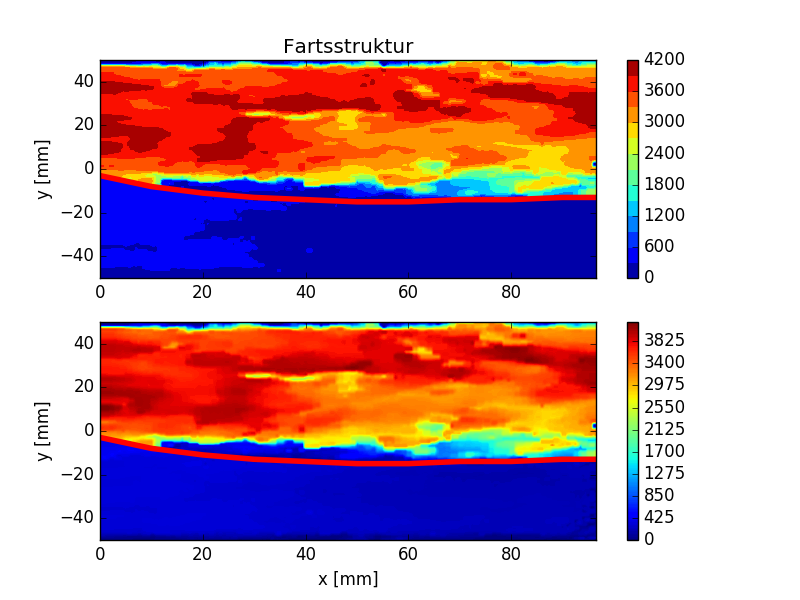
\includegraphics[width=0.6\textwidth]{problem_b}
\caption{Fartstruktur i hennholdsvis luft og vann.}
\label{fig:problem_b_contour_fig}
\end{figure}


\section*{c$)$}
\begin{figure}[H]
\centering
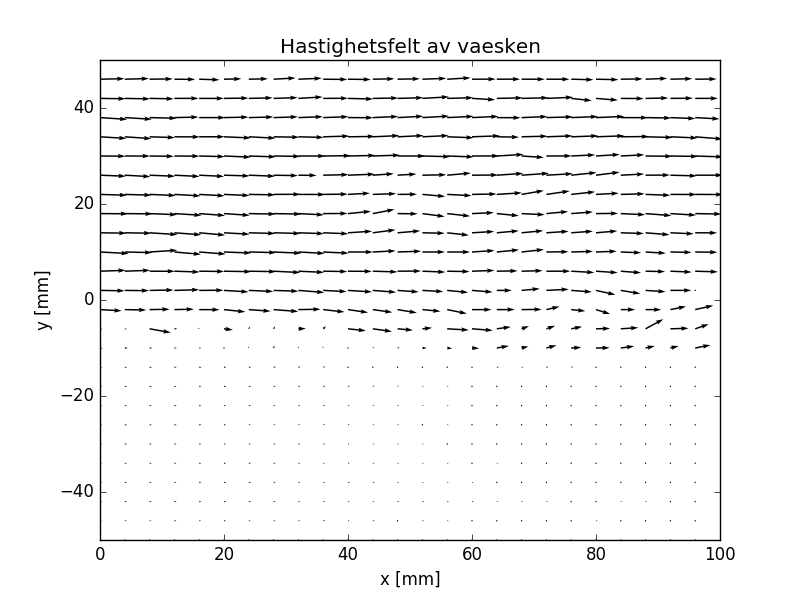
\includegraphics[width=0.6\textwidth]{problem_c_1}
\caption{Fordi hastigheten er så liten i vannet i forhold til i lufta er det vanskelig å se vektorpilene.}
\label{fig:problem_b_vector_fig}
\end{figure}

\section*{d$)$}
Divergensen til $\vec{v}$ er gitt ved
\begin{equation}
\nabla\cdot\vec{v} = \frac{\partial}{\partial x}u + \frac{\partial}{\partial y}v + \frac{\partial}{\partial z}w,
\end{equation}
men måten eksperimentet er satt opp på gir $\frac{\partial}{\partial z}w = 0$.
Imkompressibel vil si at når man følger en fluidpartikkel gjennom et hastighetsfelt vil den ha konstant tetthet
\begin{equation}
\frac{D\rho}{dt} = 0.
\end{equation}
Derav fra kontinuitetsligningen har vi at
\begin{equation}
\frac{D\rho}{dt} + \rho\nabla\cdot\vec{v} = 0,
\end{equation}
hvor vi har at $\nabla\cdot\vec{v} = 0$ for imkomprissibelt fluid. Dette betyr at $\nabla\cdot\vec{v} = 0$
\begin{equation}
\frac{\partial}{\partial z}w = -\bigg(\frac{\partial}{\partial x}u + \frac{\partial}{\partial y}v\bigg)
\end{equation}

\section*{e$)$}
Virvlingen til $\vec{v}$ er gitt ved
\begin{equation}
\nabla\cdot\vec{v} = \begin{vmatrix}\hat{i}&\hat{j}&\hat{k}\\\partial_{x}&\partial_{y}&\partial_{z}\\u&v&w\end{vmatrix}. 
\end{equation}
Som gir
\begin{equation}
\hat{k}\bigg(\frac{\partial}{\partial_{x}}v - \frac{\partial}{\partial_{y}}u \bigg),
\end{equation}
altså komponenten \textit{normalt på xy-planet}.
\section*{f$)$}

\section*{g$)$}

\section*{Kildekode}
\hypertarget{sourcecode}{}
\lstinputlisting[language=Python]{code.py}


\end{document}

